%
% Thesis Style 用サンプル TeX
%
% コンパイルには llmk を用いること.
%
% 両面印刷する時は twoside にする
%
\documentclass[12pt,twoside]{jbook}
\usepackage{csg-thesis}
\usepackage[dvipdfmx]{graphicx}
\usepackage{url}
\usepackage{boxedminipage}


\newcommand{\pyrevise}{\texttt{pyrevise}}

\begin{document}

% 題目
% 適当に改行(\\)で区切って見やすくする
\title{%
  pyrevise: プログラミング教育を対象にした生成AIによるエラー文の理解支援
}

% 学位(学部と大学院で変更)
\degree{学士}
% \degree{修士}

% 名前
\author{%
  城越 悠仁
}

% 提出日
\date{2025年1月30日}

% 卒業年度
\schoolyear{令和6年}

% 所属(学部と大学院で変更)
% \department{京都産業大学 コンピュータ理工学部 コンピュータサイエンス学科}
% \department{京都産業大学 コンピュータ理工学部 ネットワークメディア学科}
% \department{京都産業大学 コンピュータ理工学部 インテリジェントシステム学科}
\department{京都産業大学 情報理工学部}
% \department{京都産業大学大学院 先端情報学専攻}

% 学籍番号
\stnumber{153678}

% 指導教員(教官ではなくなった...)
\supervisor{玉田 春昭 教授}

\pagenumbering{roman}  %% ページ番号をローマ数字にする

\maketitle

%%%%%%%%%%%%%%%%%%%%%%%%%%%%%%%%%%%%%%%%%%%%%%%%%%%%%%%%%%%%%%%%%%%%%%

% 概要
\begin{abstract}
  プログラミング初学者にとって,プログラム実行時に表示されるエラー文を正確に理解し,その原因や解決方法を把握することは,学習過程における重要な課題である.
  しかし,多くの初学者はエラー文の内容やプログラム内の発生箇所を理解するのに時間がかかり,その過程で挫折してしまうケースも少なくない.
  特にエラー文が難解であったり,適切な修正方法が想像しにくい場合には,学習効率やモチベーションが大きく低下することが指摘されている.

  本研究では,この課題を解決するため,生成AIを活用したエラー文理解支援ツールを提案する.
  本ツールは,実行時のエラーメッセージとプログラムのソースコードを入力として受け取り,生成AIを用いてエラーの原因を特定し,解決策を提示する仕組みを持つ.
  生成AIによるフィードバックは,初心者でも理解しやすい形で提供されるため,エラー文に対する学習者の理解を促進し,効率的な問題解決を可能にする.

  さらに,本研究では提案ツールの有効性を検証するため,学習効率やエラー理解の深度,学習意欲への影響について評価を行った.
  その結果,本ツールはエラー修正速度の向上やエラー再発防止率の向上に寄与することが確認された.また,エラーの解決率も向上し,学習者の学習効果を高めることができることが示された.
  これらの結果から,ツール「\pyrevise」はエラー解決スキルの向上と学習の効率化に寄与することが確認された.一方で,特定のエラーへの対応やフィードバック内容の改善が今後の課題として挙げられる.
  本研究は,プログラミング教育における生成AIの活用可能性を示すものであり,教育現場での応用に向けた重要な知見を提供するものである.
\end{abstract}

% 謝辞
\begin{acknowledgments}
本稿は以下の方々なくして,存在しえなかったでしょう.研究などに対する助言や資料の提供などご指導を
してくださった玉田春昭教授.そして研究や調査に協力していただいた京都産業大学の一部学生のみなさん.心より感謝してい
ます.

\end{acknowledgments}

%%%%%%%%%%%%%%%%%%%%%%%%%%%%%%%%%%%%%%%%%%%%%%%%%%%%%%%%%%%%%%%%%%%%%%

\tableofcontents       %% 目次

%
% 目次等にはローマ数字を使い,本文開始ページを 1 ページ目にできる
% この方が見た目がきれいであるが,全体のページ数は減って見える
% ここでローマ数字に変えた場合は chapter 1 でアラビア数字に戻すこと
%

\listoffigures         %% 図目次(図がない場合は不要)
%%\listoftables          %% 表目次(表がない場合は不要)

%%%%%%%%%%%%%%%%%%%%%%%%%%%%%%%%%%%%%%%%%%%%%%%%%%%%%%%%%%%%%%%%%%%%%%

\pagenumbering{arabic}
%
% 本文
%
\chapter{はじめに}

プログラミング初学者は,学習の過程で直面するエラーや複雑な概念の理解に苦しむことが多い.
そのため,初学者はプログラミング学習に対して苦手意識を持つことが報告されている\cite{2015icce_fu}.
特に,プログラム実行時に表示されるエラーメッセージは,専門的な用語や技術的な内容を含むことが多く,初学者にとっては難解である.
この結果,エラーの原因を突き止めるための時間が長引き,学習効率が低下するだけでなく,学習意欲が低下し,最終的には挫折してしまう例も少なくない\cite{2016ipsj_makihara}.

苦手意識を持たせないために,これまでに様々な初学者のプログラミング学習支援手法が研究されている\cite{2016ipsj_makihara,2021fose_akiyama}.
例えば,エラー文を分かりやすく翻訳するツールや,視覚的なデバッグ支援システムなどが提案されている\cite{2021fose_akiyama}.
しかし,これらの多くはエラーの技術的な側面を提示するに留まり,初学者がエラーの背景や根本原因を深く理解するための支援としては十分ではない.

一方で,近年の生成AI技術の急速な発展は,教育分野において新たな可能性を提供している\cite{2023jssst_tanaka}.
生成AIは,学習者が抱える疑問に対して文脈を考慮した応答を生成し,個々の理解度に応じたサポートを提供することが可能である.
例えば,ChatGPTなどの生成AIは,数学や語学教育の場面で活用されており,学習成果の向上が確認されている\cite{2023jssst_tanaka}.
このような生成AIの技術をプログラミング教育に応用することで,初心者が感じる学習のハードルを下げるための強力なツールとなり得る.

そこで本稿では,初学者がプログラムを実行したときにエラーが発生すると,即座にフィードバックを提供するツールを提案する.
本ツールは,生成AIを活用して実行時のエラーメッセージとプログラムのソースコードを解析し,エラーの原因と解決策を学習者に提示する\cite{2023jssst_tanaka}.
これにより,学習者はエラーメッセージを理解し,独力で解決する力を養うことが期待される.
また,ツールの迅速なフィードバックにより試行錯誤の効率が向上し,学習者が実践的なスキルを身に付けるための基盤が整うと考えられる.

%%%%
\chapter{関連研究}
プログラミング初学者に対する学習支援の重要性は,多くの研究で指摘されている.
特に,エラー文の理解を促進し,学習効率を向上させる取り組みが注目されている.

近藤ら\cite{2023repit_kondo}は,初学者にとってコンパイルエラーメッセージが複雑で理解が困難である点に着目し,エラーメッセージを原因ごとに分類して提示する手法を提案した.
この手法は,エラーメッセージを段階的に解決可能な形に整理することで,学習者が効率的に問題解決を進められることを示している.
本研究の「エラー修正スピードの分析」と「エラー発生頻度の解析」において,この手法は直接的な基盤となる.

また,金澤ら\cite{2019ipsj_kanazawa}は,プログラミング編集過程の履歴を学習者自身が振り返ることで,コンパイルエラー修正を支援するツールを提案した.
この研究では,編集履歴を通じてエラー修正のプロセスを可視化することで,学習者のエラー修正能力が向上することを示している.
本研究の「修正履歴の追跡」および「エラーの再発防止率」の評価において,この履歴活用の考え方が適用されている.

これらの関連研究を踏まえ,本研究では生成AIを活用し,エラー文の理解支援に特化したツールを開発する.
本研究の独自性は,ログ機能を活用して学習者のエラー修正スピードや再発防止率などを多角的に分析する点にある.

%%%%
\chapter{提案手法}\label{sect:requirements}
\section{背景と課題}
今日の多くのプログラミング言語では,プログラム実行時にエラーが発生すると,エラーメッセージとスタックトレースが出力される.
これらはエラーの種類を示すとともに,エラー箇所の特定につながる情報を提供する.
プログラムに慣れた学習者(中級者と呼ぶ)は,エラーの種類から原因を推測し,スタックトレースからエラーの発生場所を限定することで,エラーの解消を行えるようになる.
しかし,こうしたスキルは一朝一夕に習得できるものではなく,初学者にとってはエラーの解釈が難解であり,学習の大きな障壁となる\cite{2012ies_sakakibara}.

初学者が直面する主な課題として,次の3点が挙げられる.
\begin{quote}
	\begin{enumerate}
	 \item エラーメッセージの理解不足: 技術的な内容を読み取る能力が未熟であるため,エラーの意味が分からない.
	 \item スタックトレースの解釈困難: エラーの発生箇所を特定できず,修正の手がかりを見つけられない.
	 \item 原因推測の経験不足: エラーの背景や原因を体系的に考察する力が不足している.
	\end{enumerate}
\end{quote}
これらの課題を解決するために,本稿ではプログラム実行時にエラーが発生した場合,即座にフィードバックを提供するツール\pyrevise を提案する.
本ツールは,プログラムの実行状態を監視し,エラーが発生した際に生成AI(ChatGPT)を用いてエラー内容を解析し,修正案を提示することで,初学者がエラー修正能力を向上させることを目的とする.

\section{提案するツール \pyrevise の概要}
本ツールでは,プログラムの終了ステータスとエラーメッセージを基にエラーを検出する.
多くの場合,プログラムが正常に終了した場合は終了ステータスが0となり,それ以外の場合にエラーが発生したとみなす.
そして,エラーが検出された場合,出力されたエラーメッセージとプログラムのソースコードを生成AIに与え,解決策を推薦する.
本ツールの動作フローを図\ref{fig:flowchart}に示す.

\begin{figure}[h]
  \centering
  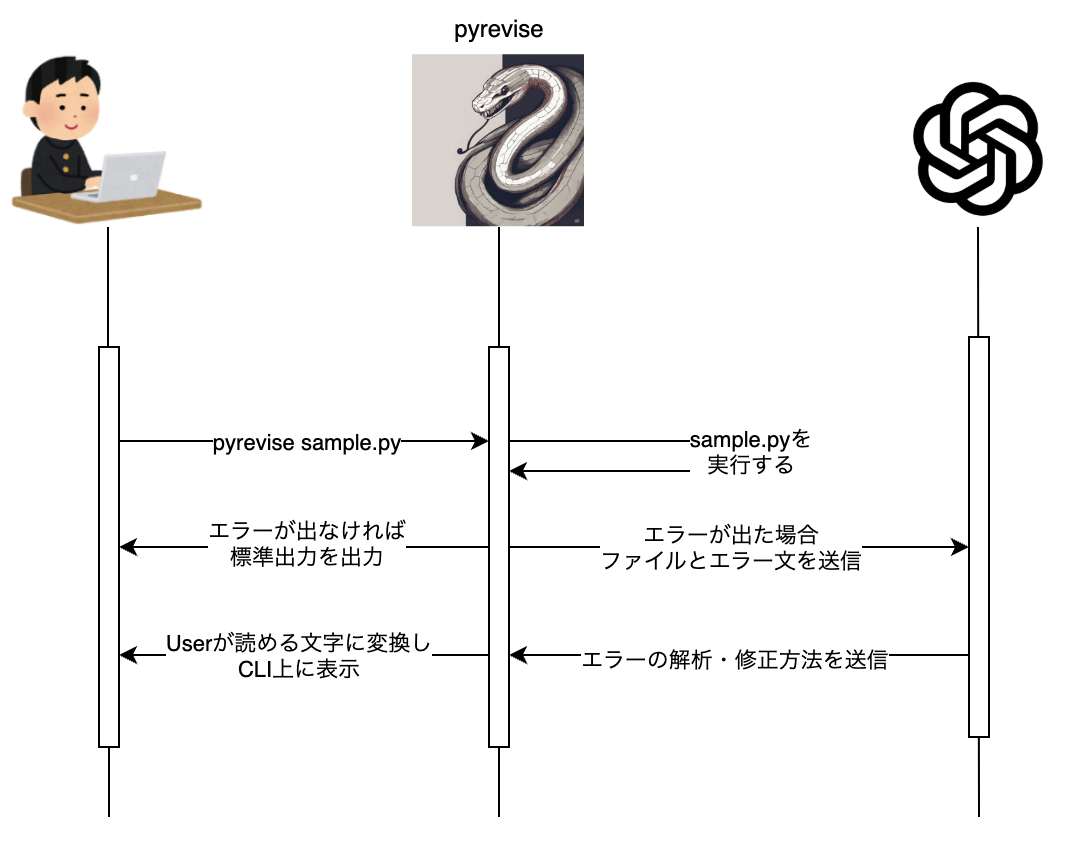
\includegraphics[width=0.8\textwidth]{images/flowchart.png}
  \caption{提案手法 \pyrevise の動作フロー}
  \label{fig:flowchart}
\end{figure}

本図は,ユーザーが\pyrevise を用いてPythonプログラムを実行する際の動作フローを示している.具体的には以下の3つのステップを経て動作する.

\begin{quote}
    \begin{enumerate}
	 \item プログラムの実行監視:
      プログラムの実行結果を監視し,終了ステータスが0以外の場合にエラーメッセージを取得する.
	 \item 生成AIとの連携:
	    エラーメッセージと関連するコードをChatGPTに送信し,修正案を生成する.
	 \item フィードバックの提示:
	    生成された修正案を学習者に提示し,エラーの原因と解決方法を明確化する.
    \end{enumerate}
\end{quote}

これにより,初学者が解釈しづらいエラーメッセージを生成AIが分かりやすく説明し,エラーの原因と解決策を提示できると期待される.
本ツールは,学習者がエラーの修正プロセスを通じて学習を深めるだけでなく,エラー解消の成功体験を通じて自己効力感を高める効果も期待される.

また,本研究において\pyrevise の有効性を検証するために必要なデータは,本ツール実行時にローカルの特定の場所にログファイルとして保存される.
保存するデータは以下の4つである.
\begin{itemize}
  \item 実行時間
  \item 実行したファイルのパス
  \item 実行処理時間
  \item ファイルの実行結果
\end{itemize}

これらのデータが保存されたログファイルを,Google Drive上にアップロードしてもらい,様々な評価実験を行う.


%%%%
\chapter{試作システム \pyrevise}

第\ref{sect:requirements}章で述べた内容を基に,エラー文理解支援ツール\pyrevise を作成した\footnote{\url{https://github.com/tamadalab/pyrevise/}}.
本ツールは,プログラムの実行中に発生するエラーを監視し,その内容を解析した上で解決策を提示するものである.
これにより,初学者がエラーメッセージを理解できないという障壁を乗り越え,プログラムの修正スキルを効率的に向上させることを目的としている.
本章では,ツールの動作概要と構成,実行例,具体的な出力結果について説明する.

\section{ツールの構成と動作}
\pyrevise は,コマンドラインから操作可能なシンプルなツールとして設計されている.
本ツールは,Pythonスクリプトを引数に指定して実行することで動作し,以下の3つの主要機能を備えている.

まず,プログラムの実行中にエラーが発生すると,ツールがそのエラーメッセージをリアルタイムでキャプチャする.
この段階では,Pythonのsubprocessモジュールを使用し,標準エラー出力(stderr)を監視することでエラー内容を取得する.
終了ステータスが0以外の場合,ツールは次のステップに進み,エラーメッセージを解析する.

次に,検出されたエラーメッセージと関連するソースコードのスニペットをChatGPT APIに送信する.
ここでは,生成AIに対するプロンプト設計が重要な役割を果たす.本ツール内で使用するプロンプトは図\ref{fig:prompt}に示す通りである.
適切なプロンプトを通じて,エラーの背景情報や修正方針をAIに正確に伝え,精度の高い修正案を生成する.
このプロセスにより,初学者にも理解しやすい形式で原因説明と修正案が提供される.

最後に,生成された修正案をターミナル上で表示する.
この修正案には,エラーの詳細な原因,修正手順,修正コード例が提示される.
これにより,学習者はエラーの解決方法だけでなく,将来的な同様の問題への対処方法も学ぶことができる.

\begin{figure}
  \centering
  {\footnotesize
  \begin{boxedminipage}{1.02\columnwidth}
以下のプログラムコードにエラーが見つかりました:\\
\verb!<プログラムコード>!\\
エラーメッセージ:\\
\verb!<エラーメッセージ>!\\
このエラーの原因と修正提案を教えてください.
  \end{boxedminipage}}
  \caption{ChatGPT に与えたプロンプト}\label{fig:prompt}
  \vspace{0.2cm}
\end{figure}

\section{ツールの実行例}
図\ref{fig:program} は,3行目でリストの範囲外を参照するため,\texttt{IndexError} が発生するプログラムである.
このプログラムを \pyrevise で実行した結果を 図\ref{fig:result} に示す.

\begin{figure}[t]
  {\footnotesize
  \begin{boxedminipage}{1.02\columnwidth}
\verb!  1: def raise_error():!\\
\verb!  2:     my_list = [1, 2, 3]!\\
\verb!  3:     print(my_list[5])!\\
\verb!  4: if __name__ == "__main__":!\\
\verb!  5:     raise_error()!
\end{boxedminipage}}
  \caption{プログラム例(\texttt{index\_error.py})}\label{fig:program}
  \vspace{0.2cm}
  {\footnotesize
  \begin{boxedminipage}{1.02\columnwidth}
エラーメッセージ:\\
\verb!Traceback (most recent call last):!\\
\verb!  File "index_error.py", line 7, in <module>!\\
\verb!    raise_index_error()!\\
\verb!  File "index_error.py", line 3, in raise_error!\\
\verb!    print(my_list[5])!\\
\verb!          ~~~~~~~^^^!\\
\verb!IndexError: list index out of range!\\
エラー原因:\\
ここで発生しているエラーは「IndexError」で,それは配列の範囲外のインデックスを参照しようとしたときに生じるものです.具体的には,my\_list には3つの要素(0, 1, 2番目のインデックス)しかないのに,5番目のインデックスを参照しようとしたために起きています.\\
修正提案:\\
my\_listから存在するインデックス(0, 1, 2)を参照するように変更することで,このエラーは解決します.以下に修正後のコードを示します:\\
... 後略(修正コード例が提示される)...
% ```python
% def raise_index_error():
%     my_list = [1, 2, 3]
%     print(my_list[2])  # Change index from 5 to 2
% if __name__ == "__main__":
%     raise_index_error()
% ```

% なお,存在しないインデックスを参照しようとしたときにエラーを回避する方法として,例外処理を用いる方法もあります:

% ```python
% def raise_index_error():
%     my_list = [1, 2, 3]
%     try:
%         print(my_list[5])
%     except IndexError:
%         print("IndexError occurred. Index out of range.")

% if __name__ == "__main__":
%     raise_index_error()
% ```
% このコードは,IndexErrorが発生した場合にエラーメッセージを表示するようになっています.
  \end{boxedminipage}}
  \caption{\pyrevise での \texttt{index\_error.py} の実行結果}\label{fig:result}
\end{figure}
この修正案では,エラーの原因を簡潔に説明した上で,具体的なコード例を示している.
これにより,学習者はエラーを修正するだけでなく,同じエラーを防ぐためのコーディング方法も学ぶことができる.

%%%%
\chapter{評価実験}\label{sect:evaluation}
提案するツール\pyrevise の有効性を検証するために,プログラミング学習者を対象とした評価実験を実施した.
本実験は,制限時間を設け,初学者向けのプログラミング学習を行う学習者を対象に行われた.
本実験では,ツールがエラー修正プロセスや学習効果に与える影響を多角的に分析し,以下の4つの指標に基づいて評価を行った.
\begin{itemize}
  \item エラー修正スピードの分析
  \item エラー発生頻度の解析
  \item エラー解決率の分析
  \item エラーの再発防止率
\end{itemize}

本研究は,プログラミング初学者を対象とした実験である.
そのため,被験者として,京都産業大学の一年生が必修で受講する基礎プログラミング演習を履修する学生を対象に実験を行なった.

\section{エラー修正スピードの分析}
本評価項目では,学習者がエラーを修正するまでに要した時間を計測し,ツールの有用性を検証した.
具体的には,エラーが発生してから修正が完了するまでの実行時間とエラー文を比較することで,ツールがエラー解決のスピードに与える影響を測定した.

ツールを使用し続けることで学習者がエラーの修正時間が短くなるかどうかを検証する.
ツールがエラーメッセージの解釈や修正方法の提示を迅速に行うことで,学習者がエラー解決に要する時間を大幅に短縮できることが期待される.
この指標は,ツールがエラー修正プロセスの効率化に寄与する度合いを示すものである.

\section{エラー発生頻度の解析}
学習者がどのようなエラーに頻繁に直面しているかを明らかにするため,エラー文とその発生回数を記録した.
本分析では,各エラー文の頻度を解析し,学習者が特に苦労しているエラーの傾向を可視化することを目的としている.

記録されたデータを基に,頻発するエラーを特定することで,ツールのさらなる改良や学習コンテンツの設計に役立てることができる.
例えば,特定のエラーが頻繁に発生している場合,そのエラーに対してより適切な修正案や説明を提示することで,学習者の負担を軽減することが可能である.

\section{エラー解決率の分析}
エラー解決率は,ツールが問題解決にどの程度寄与しているかを示す重要な指標である.
本評価では,実行されたプログラムのうち,エラーを完全に修正して再実行に成功した割合を計測した.
また,同じファイルパスにおけるエラーの減少傾向を追跡し,最終的にプログラムが正常に動作するまでのプロセスを分析した.

エラー解決率の高さは,ツールが学習者にとって効果的な支援を提供していることを示す指標である.
また,修正案が適切であるほどエラー解決率が向上するため,この結果はツールの設計や生成AIのプロンプト設計の妥当性を評価する上でも重要な意味を持つ.

\section{エラーの再発防止率}
エラーの再発防止率は,学習者が同じ種類のエラーを再度発生させる割合を測定することで評価した.
過去に発生したエラーと同じエラーが再発しているかを追跡し,学習者がエラーからどの程度学び,同じミスを繰り返さなくなったかを確認した.

本指標は,学習者がエラー修正の過程でどれだけ深い理解を得ているかを評価するものであり,ツールが学習者の長期的なスキル向上にどの程度寄与しているかを示す.
また,再発するエラーが減少することで,ツールが学習者の自己解決能力を向上させる効果を測定することが可能である.


\chapter{結果}
第\ref{sect:evaluation}章での評価指標を基に実験を行った結果を本章で示す.

\section{エラー修正スピードの分析}
エラーが発生してから修正が完了するまでに要した時間を分析した.図\ref{fig:fix}に示すように,エラーの修正に要する時間にはばらつきが見られるものの,
多くのエラーが短時間で修正されていることがわかる.
特に,200秒以内に修正が完了するエラーが最も多く,全体の修正速度において改善が確認された.

\begin{figure}[h]
  \centering
  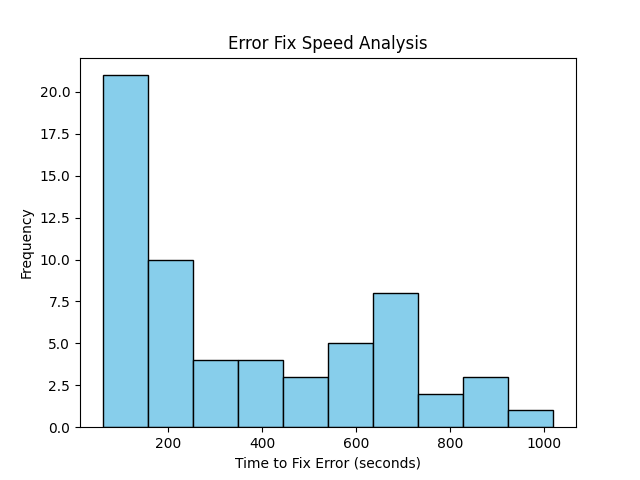
\includegraphics[width=0.8\textwidth]{images/fix_speed_analysis.png}
  \caption{エラー修正スピードの推移}
  \label{fig:fix}
\end{figure}

この結果は,提案手法がエラーメッセージを解釈しやすく変換し,学習者が迅速に解決方法を見つけられるよう支援したことを示唆している.
また,修正時間の短縮は学習者がツールを使用することで,エラー解決に慣れ,効率的な手順を身につけたことが原因と考えられる.

\section{エラー発生頻度の解析}
本ツールのエラー発生頻度の結果を図\ref{fig:frequency}に示す.
この図では,頻度の高いエラーが上位10種類表示されており,IndexError や SyntaxError が特に多く発生していることがわかった.
これらのエラーは初学者にとってよくある典型的なエラーであり,スタックトレースやメッセージの理解が不十分な場合に解決が難しいとされる.

\begin{figure}[h]
  \centering
  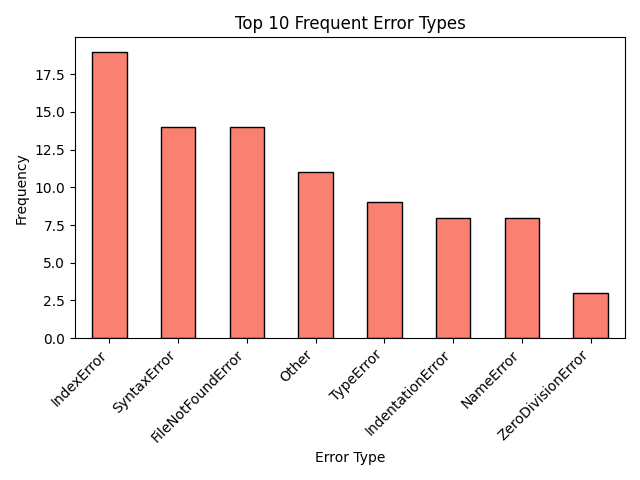
\includegraphics[width=0.8\textwidth]{images/frequency_analysis.png}
  \caption{エラー発生頻度について}
  \label{fig:frequency}
\end{figure}

これにより,ツールがこれら頻発エラーに対して適切な修正案を提示することが,学習者の理解を深め,エラー解決のプロセスを支援する重要な要素であることが確認された.


\section{エラー解決率の分析}
本節では,プログラムのうち,エラーが完全に修正され再実行に成功したケースを計測した.
図\ref{fig:resolution} に示すように,エラー修正に成功したプログラムがエラー修正に失敗したプログラムよりも多いことが確認された.
これにより,本ツールが学習者にエラーの解決方法を的確に提示し,エラー解決率を向上させる効果があることが示唆された.

\begin{figure}[h]
  \centering
  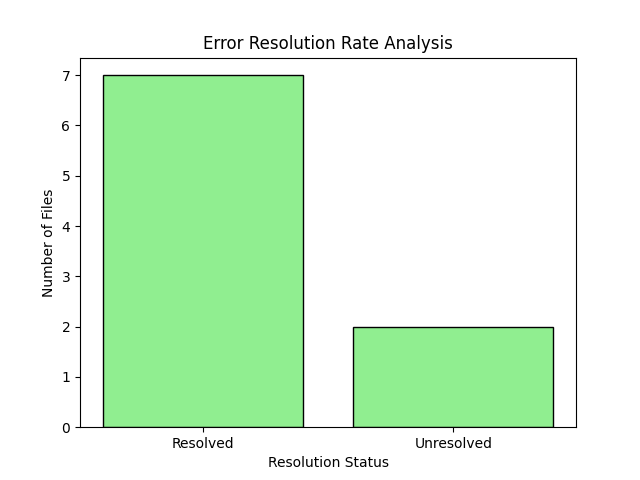
\includegraphics[width=0.8\textwidth]{images/resolution_analysis.png}
  \caption{エラーの解決率の割合}
  \label{fig:resolution}
\end{figure}

この結果は,生成AIによるフィードバックが有効であり,学習者が提示された修正案を実行することでエラーを効果的に修正できたことを示している.
また,解決に至らなかったケースでは,複雑なロジックエラーや修正案の不十分さが影響している可能性が考えられる.


\section{エラーの再発防止率}
本ツールのエラー再発防止率の結果を図\ref{fig:recurrence}に示す.
この図から,約66%のケースで同じエラーが再発していないことがわかる.一方で,34%のケースでは再発が見られた.

\begin{figure}[h]
  \centering
  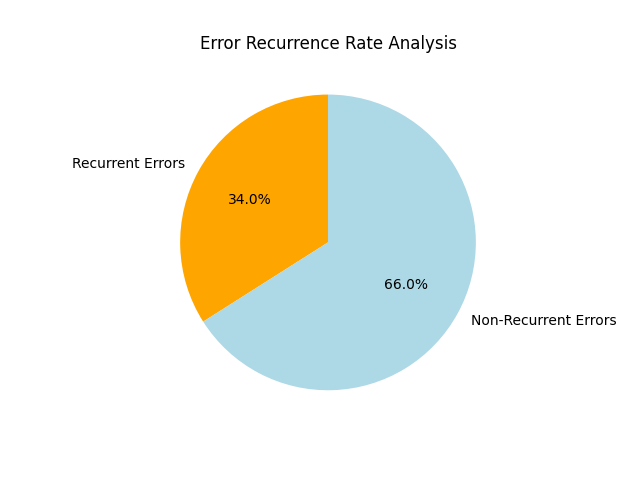
\includegraphics[width=0.8\textwidth]{images/recurrence_analysis.png}
  \caption{エラーの再発防止率の推移}
  \label{fig:recurrence}
\end{figure}

エラーが再発しないケースが多いことは,ツールが学習者の理解を促進し,同じ種類のエラーを回避する力を養っていることを示している.
しかし,再発が見られたケースについては,提示された修正案が不十分であったか,学習者がその内容を正しく理解できなかった可能性が考えられる.


%%%%
\chapter{まとめ}
以上の分析結果を総合すると,提案するツール「\pyrevise」は,エラー解決スピードの向上や学習者のスキル向上に寄与していることが確認された.
特に,頻発するエラーに対する支援や,同じエラーの再発防止において一定の効果が見られた.
一方で,再発が見られたケースや解決に至らなかったケースについては,さらなる改善が必要であると考えられる.
今後の改良として,以下の点が挙げられる. 
\begin{itemize} 
  \item より具体的で理解しやすい修正案の提示 
  \item 学習者の理解度に応じたフィードバック内容の最適化 
  \item 追加の学習リソースへのリンク提供による補完 
\end{itemize}

これにより,ツールが学習者にとってより効果的な支援を提供できると期待される.

%%%%%%%%%%%%%%%%%%%%%%%%%%%%%%%%%%%%%%%%%%%%%%%%%%%%%%%%%%%%%%%%%%%%%%

%
% 参考文献は直接書いてもいいが,bibtex を使うと便利
%  (1)このサンプルを platex にかける
%  (2)jbibtex thesis
%  (3)さらに platex にかける
%  (4)もう何回か platex にかける
%
\bibliographystyle{csg-thesis}
\bibliography{thesis.bib}

%%%%%%%%%%%%%%%%%%%%%%%%%%%%%%%%%%%%%%%%%%%%%%%%%%%%%%%%%%%%%%%%%%%%%%

% 付録が必要ならつける
\appendix
% \chapter{プログラム例}


\end{document}
